\documentclass[handout]{beamer}

\usepackage{tikz}
\usetikzlibrary{quantikz2, backgrounds}
\usepackage{graphicx}
\usepackage{subcaption}

\usetikzlibrary{decorations.markings}

%\title{T-State cultivation : circuit designs}
\title{Steane Code : superdense code cycle}
\author{Dynerowicz S.}
\date{}

% Taken from https://tex.stackexchange.com/questions/126119/tex-custom-arrow-with-oplus-symbol
\makeatletter
\pgfarrowsdeclare{oplus}{oplus}{%
  \pgfarrowsleftextend{+-.5\pgflinewidth}
  \pgfutil@tempdima=0.4pt%
  \advance\pgfutil@tempdima by.2\pgflinewidth%
  \pgfutil@tempdimb=9\pgfutil@tempdima\advance\pgfutil@tempdimb by.5\pgflinewidth
  \pgfarrowsrightextend{+\pgfutil@tempdimb}%
}{%
  \pgfutil@tempdima=0.4pt%
  \advance\pgfutil@tempdima by.2\pgflinewidth%
  \pgfsetdash{}{+0pt}%
  \pgfpathcircle{\pgfqpoint{4.5\pgfutil@tempdima}{0bp}}{4.5\pgfutil@tempdima}%
  \pgfpathmoveto{\pgfqpoint{0bp}{0bp}}%
  \pgfpathlineto{\pgfqpoint{9\pgfutil@tempdima}{0bp}}%
  \pgfpathmoveto{\pgfqpoint{4.5\pgfutil@tempdima}{4.5\pgfutil@tempdima}}%
  \pgfpathlineto{\pgfqpoint{4.5\pgfutil@tempdima}{-4.5\pgfutil@tempdima}}%
  \pgfusepathqstroke
}
\makeatother

\tikzstyle{quantumR}=[red!75!black!50]
\tikzstyle{quantumB}=[blue!75!black!50]
\tikzstyle{quantumG}=[green!75!black!50]
\tikzstyle{quantumY}=[yellow!95!black!75]

\tikzstyle{data}=[circle, fill=black, text=white]
\tikzstyle{meas}=[circle, fill=white, draw=black, ultra thick]
\tikzstyle{stabilizer}=[draw=black]

\tikzstyle{interact}=[line width=1.25pt, shorten <= 8pt, shorten >= 12pt, Circle-oplus]
\tikzstyle{partner}=[line width=1.25pt, shorten <= 8pt, shorten >= 12pt, Circle-oplus]
\tikzstyle{collect}=[-stealth, line width=2pt]
\tikzstyle{error}=[shorten <= 5pt, shorten >= 5pt, stealth-stealth, line width=2pt]
\tikzstyle{entanglement}=[decorate, ultra thick,
	decoration={snake, pre length=5pt, post length=5pt, amplitude=0.5mm, segment length=2.5mm}
]

\newcommand{\Op}[1]{{\bf #1}}
\newcommand{\kett}[1]{\ket{\mbox{\tt #1}}}
\newcommand{\wn}{\wireoverride{n}}

\begin{document}
	\begin{frame}
		\titlepage
	\end{frame}

	\begin{frame}[fragile]
		\frametitle{Theory --- Bell states}
		\begin{itemize}
			\item A Bell pair "encodes" $2$ classical bits (denoted {\tt z}, {\tt x} $\in \{{\tt 0}, {\tt 1}\}$)
		\end{itemize}
		\pause
		\begin{minipage}{0.985\textwidth}
			\centering
			\begin{quantikz}[column sep=0.5cm]
				\lstick{\kett{z}} & \gate{\Op{H}} & \ctrl{1}\slice{} & \midstick[2]{
					$\frac{\kett{0x} + (-1)^{\tt z}\kett{1$\bar{\tt x}$}}{\sqrt{2}}$
				} \slice{} & \ctrl{1} & \gate{\Op{H}} & \meter{} & \setwiretype{c}\rstick{\tt z} \\
				\lstick{\kett{x}} && \targ{} && \targ{} && \meter{} & \setwiretype{c}\rstick{\tt x}
			\end{quantikz}
		\end{minipage}
		\pause
		\begin{minipage}{0.4\textwidth}
			\centering
			{\renewcommand{\arraystretch}{1.75}
				\begin{tabular}{c|c|c}
					\tt z & \tt x & $\ket{\beta_{\scriptscriptstyle\tt zx}}$ \\\hline\hline
					\tt 0 & \tt 0 & $\frac{\kett{00} + \kett{11}}{\sqrt{2}}$ \\\hline
					\pause
					\tt 0 & \tt 1 & $\frac{\kett{01} + \kett{10}}{\sqrt{2}}$ \\\hline
					\pause
					\tt 1 & \tt 0 & $\frac{\kett{00} - \kett{11}}{\sqrt{2}}$ \\\hline
					\tt 1 & \tt 1 & $\frac{\kett{01} - \kett{10}}{\sqrt{2}}$
				\end{tabular}
			}
		\end{minipage}
		\pause
		\begin{minipage}{0.585\textwidth}
			\centering
			\scalebox{0.85}{
				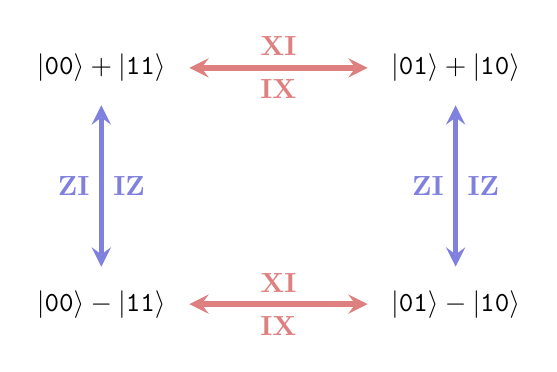
\begin{tikzpicture}
					\coordinate (b00) at (0.0,3.0);
					\coordinate (b01) at (4.5,3.0);
					\coordinate (b10) at (0.0,0.0);
					\coordinate (b11) at (4.5,0.0);
	
					\node (B00) at (b00) {$\kett{00} + \kett{11}$};
					\onslide<7->{
						\node (B01) at (b01) {$\kett{01} + \kett{10}$};
					}
					\onslide<8->{
						\node (B10) at (b10) {$\kett{00} - \kett{11}$};
					}
					\onslide<9->{
						\node (B11) at (b11) {$\kett{01} - \kett{10}$};
					}

					\onslide<7->{
						\draw[error, quantumR] (B00) --
							node[above, quantumR] {\Op{XI}}
							node[below, quantumR] {\Op{IX}} (B01);
					}
					\onslide<8->{
						\draw[error, quantumB] (B00) --
							node[left, quantumB] {\Op{ZI}}
							node[right, quantumB] {\Op{IZ}} (B10);
					}
					\onslide<9->{
						\draw[error, quantumR] (B11) --
							node[above, quantumR] {\Op{XI}}
							node[below, quantumR] {\Op{IX}} (B10);
						\draw[error, quantumB] (B11) --
							node[left, quantumB] {\Op{ZI}}
							node[right, quantumB] {\Op{IZ}} (B01);
					}
				\end{tikzpicture}
			}
		\end{minipage}
%		\begin{tikzpicture}[remember picture, overlay]
%			\node[anchor=south west, xshift=8pt, yshift=2pt, font=\tiny] at (current page.south west) {
%				\href{https://algassert.com/crumble#circuit=Q(1,1)0;Q(1,2)1;Q(1.5,1.5)2;Q(2,1)3;Q(2,2)4;Q(3,3)5;Q(3,4)6;Q(3.5,3.5)7;Q(4.5,3.5)8;Q(5,3)9;Q(5,4)10;TICK;R_8;RX_7_2;TICK;CX_7_8;TICK;CX_7_5_8_9_2_0;TICK;CX_7_6_8_10_2_3;TICK;CX_6_7_10_8_2_1;TICK;CX_9_8_5_7_2_4;TICK;CX_7_8;TICK;M_8;MX_7_2;TICK;R_2;TICK;TICK;CX_0_2;TICK;CX_3_2;TICK;CX_1_2;TICK;CX_4_2;TICK;TICK;M_2}
%				{\underline{Click here to open the circuits in Crumble}}
%				};
%		\end{tikzpicture}
	\end{frame}

%	\begin{frame}
%		\frametitle{Two configurations for teleportation}
%		\begin{itemize}
%			\item Rationale: provide enough ancillas to perform
%			\begin{itemize}
%				\item Superdense syndrome measurement for the Steane Code
%				\item Double-check in the cultivation stage
%				\item No measuring data qubits for syndrome purposes
%			\end{itemize}
%		\end{itemize}
%		\vspace{0.4cm}
%		\centering
%		\begin{figure}
%			\begin{subfigure}[b]{0.485\textwidth}
%				\centering
%				\scalebox{0.45}{
%					\begin{tikzpicture}
%						% Data qubits of the Steane Code
%						\coordinate (q1) at ( 2,-4);
%						\coordinate (q2) at (-2,-4);
%						\coordinate (q3) at ( 2,-2);
%						\coordinate (q4) at ( 4,-4);
%						\coordinate (q5) at ( 4, 0);
%						\coordinate (q6) at ( 0, 0);
%						\coordinate (q7) at ( 0,-2);
%		
%						% Extra data qubits for forming GHZ states
%						\coordinate (dR) at ( 4,-2);
%						\coordinate (dG) at ( 0, 0);
%						\coordinate (dB) at ( 0,-4);
%						\coordinate (a0) at ( 1,-1);
%						\coordinate (a1) at ( 3,-1);
%						\coordinate (a2) at (-1,-3);
%						\coordinate (a3) at ( 1,-3);
%						\coordinate (a4) at ( 5,-1);
%						\coordinate (a5) at ( 3,-3);
%		
%						% Plaquettes of the Steane Code
%						\fill[quantumR] (q5) -- (q3) -- (q1) -- (q4) -- (dR) -- cycle;
%						\fill[quantumG] (q6) -- (dG) -- (q5) -- (q3) -- (q7) -- cycle;
%						\fill[quantumB] (q2) -- (q7) -- (q3) -- (q1) -- (dB) -- cycle;
%			
%						% Plaquettes of the Surface Code
%						\fill[quantumR] (2,-6) -- (4, -6) -- (4, -7) -- (2, -7);
%						\fill[quantumR] (6,-6) -- (8, -6) -- (8, -7) -- (6, -7);
%						\fill[quantumB] (0,-6) -- (2, -6) -- (2, -7) -- (0, -7);
%						\fill[quantumB] (4,-6) -- (6, -6) -- (6, -7) -- (4, -7);
%						\fill[quantumB] (6, -6) arc[start angle=180, end angle=0, radius=1.0] -- (8, -6) -- cycle;
%						\fill[quantumB] (8, -6) arc[start angle= 90, end angle=0, radius=1.0] -- (8, -7) -- cycle;
%			
%						\fill[quantumB, opacity=0.25] (2,-4) -- (4, -4) -- (4, -6) -- (2, -6);
%						\filldraw[quantumB, opacity=0.25] (-2,-4) to[bend left=30] (0,-6) to[bend left=30] (-2,-4);
%		
%						\node[data] at ( 2, 0) {\phantom{o}};
%						\node[data] at ( 4,-2) {\phantom{o}};
%						\node[data] at ( 0,-4) {\phantom{o}};
%		
%						\node[data] at (q1) {\large $\mathbf{1}$};
%						\node[data] at (q2) {\large $\mathbf{2}$};
%						\node[data] at (q3) {\large $\mathbf{3}$};
%						\node[data] at (q4) {\large $\mathbf{4}$};
%						\node[data] at (q5) {\large $\mathbf{5}$};
%						\node[data] at (q6) {\large $\mathbf{6}$};
%						\node[data] at (q7) {\large $\mathbf{7}$};	
%						\node[circle, draw=yellow!95!black!75, line width=2pt] at (q7) {\phantom{o}};
%
%						\foreach \x in { 1, 3, 5}{ \node[meas] at (\x,-1) {}; }
%						\foreach \x in {-1, 1, 3}{ \node[meas] at (\x,-3) {}; }
%						\foreach \x in {-1, 3}{ \node[meas, opacity=0.25] at (\x,-5) {}; }
%		
%						\foreach \x in {0, 2, 4, 6, 8}{ \node[data] at (\x, -6) {\phantom{o}}; }
%					\end{tikzpicture}
%				}
%				\caption{Layout $1$}
%			\end{subfigure}
%			\hfill
%			\begin{subfigure}[b]{0.485\textwidth}
%				\centering
%				\scalebox{0.45}{
%					\begin{tikzpicture}
%						% Data qubits of the Steane Code
%						\coordinate (q1) at ( 2,-4);
%						\coordinate (q2) at (-2,-4);
%						\coordinate (q3) at ( 2,-2);
%						\coordinate (q4) at ( 4,-4);
%						\coordinate (q5) at ( 2, 0);
%						\coordinate (q6) at (-2, 0);
%						\coordinate (q7) at ( 0,-2);
%		
%						% Extra data qubits for forming GHZ states
%						\coordinate (dR) at ( 4,-2);
%						\coordinate (dG) at ( 0, 0);
%						\coordinate (dB) at ( 0,-4);
%						\coordinate (a0) at (-1,-1);
%						\coordinate (a1) at ( 1,-1);
%						\coordinate (a2) at (-1,-3);
%						\coordinate (a3) at ( 1,-3);
%						\coordinate (a4) at ( 3,-1);
%						\coordinate (a5) at ( 3,-3);
%		
%						% Plaquettes of the Steane Code
%						\fill[quantumR] (q5) -- (q3) -- (q1) -- (q4) -- cycle;
%						\fill[quantumG] (q6) -- (dG) -- (q5) -- (q3) -- (q7) -- cycle;
%						\fill[quantumB] (q2) -- (q7) -- (q3) -- (q1) -- (dB) -- cycle;
%			
%						% Plaquettes of the Surface Code
%						\fill[quantumR] (2,-6) -- (4, -6) -- (4, -7) -- (2, -7);
%						\fill[quantumR] (6,-6) -- (8, -6) -- (8, -7) -- (6, -7);
%						\fill[quantumB] (0,-6) -- (2, -6) -- (2, -7) -- (0, -7);
%						\fill[quantumB] (4,-6) -- (6, -6) -- (6, -7) -- (4, -7);
%						\fill[quantumB] (6,-6) arc[start angle=180, end angle=0, radius=1.0] -- (8, -6) -- cycle;
%						\fill[quantumB] (8,-6) arc[start angle= 90, end angle=0, radius=1.0] -- (8, -7) -- cycle;
%
%						\fill[quantumB, opacity=0.25] (2,-4) -- (4, -4) -- (4, -6) -- (2, -6);
%						\filldraw[quantumB, opacity=0.25] (-2,-4) to[bend left=30] (0,-6) to[bend left=30] (-2,-4);
%		
%						\node[data] at ( 0, 0) {\phantom{o}};
%						\node[data] at ( 4,-2) {\phantom{o}};
%						\node[data] at ( 0,-4) {\phantom{o}};
%		
%						\node[data] at (q1) {\large $\mathbf{1}$};
%						\node[data] at (q2) {\large $\mathbf{2}$};
%						\node[data] at (q3) {\large $\mathbf{3}$};
%						\node[data] at (q4) {\large $\mathbf{4}$};
%						\node[data] at (q5) {\large $\mathbf{5}$};
%						\node[data] at (q6) {\large $\mathbf{6}$};
%						\node[data] at (q7) {\large $\mathbf{7}$};
%						\node[circle, draw=yellow!95!black!75, line width=2pt] at (q7) {\phantom{o}};
%
%						\foreach \x in {-1, 1, 3}{
%							\foreach \y in {-1, -3}{
%								\node[meas] at (\x,\y) {};
%							}
%						}
%						\foreach \x in {-1, 3}{ \node[meas, opacity=0.25] at (\x,-5) {}; }
%		
%						\foreach \x in {0, 2, 4, 6, 8}{ \node[data] at (\x, -6) {\phantom{o}}; }
%					\end{tikzpicture}
%				}
%				\caption{Layout $2$}
%			\end{subfigure}
%		\end{figure}
%	\end{frame}

	\begin{frame}
		\frametitle{Requirements --- Superdense Syndrome Measurement}
		\begin{itemize}
			\item Superdense code cycle requires $2$ ancillas per plaquette
			\begin{itemize}
				\item $+3$ data qubits (used to form GHZ states, not measured)
				\item handling GHZ state requires $+2$ CNOTs per plaquette
				\item separating Z/X flows requires $+1$ CNOT per plaquette
			\end{itemize}
		\end{itemize}
		\vspace{0.4cm}
		\centering
		\scalebox{0.75}{
			\begin{tikzpicture}
				% Data qubits of the Steane Code
				\coordinate (q1) at ( 2,-4);
				\coordinate (q2) at (-2,-4);
				\coordinate (q3) at ( 2,-2);
				\coordinate (q4) at ( 4,-4);
				\coordinate (q5) at ( 4, 0);
				\coordinate (q6) at ( 0, 0);
				\coordinate (q7) at ( 0,-2);

				% Extra data qubits for forming GHZ states
				\coordinate (dR) at ( 4,-2);
				\coordinate (dG) at ( 2, 0);
				\coordinate (dB) at ( 0,-4);
				\coordinate (a0) at ( 1,-1);
				\coordinate (a1) at ( 3,-1);
				\coordinate (a2) at (-1,-3);
				\coordinate (a3) at ( 1,-3);
				\coordinate (a4) at ( 5,-1);
				\coordinate (a5) at ( 3,-3);

				% Plaquettes of the Steane Code
				\fill[quantumR] (q5) -- (q3) -- (q1) -- (q4) -- (dR) -- cycle;
				\fill[quantumG] (q6) -- (dG) -- (q5) -- (q3) -- (q7) -- cycle;
				\fill[quantumB] (q2) -- (q7) -- (q3) -- (q1) -- (dB) -- cycle;

				\draw[entanglement] (dG) -- (a0);
				\draw[entanglement] (dG) -- (a1);
				\draw[entanglement] (dB) -- (a2);
				\draw[entanglement] (dB) -- (a3);
				\draw[entanglement] (dR) -- (a4);
				\draw[entanglement] (dR) -- (a5);

				\only<2>{
					\draw[interact] (a0) -- (q6);
					\draw[interact] (a0) -- (q7);
					\draw[interact] (a1) -- (q5);
					\draw[interact] (a0) -- (q3);

					\draw[interact] (a2) -- (q2);
					\draw[interact] (a2) -- (q7);
					\draw[interact] (a3) -- (q3);
					\draw[interact] (a3) -- (q1);

					\draw[interact] (a4) -- (q5);
					\draw[interact] (a5) -- (q3);
					\draw[interact] (a5) -- (q1);
					\draw[interact] (a5) -- (q4);
				}

				\node[data] at (dR) {\phantom{o}};
				\node[data] at (dG) {\phantom{o}};
				\node[data] at (dB) {\phantom{o}};

				\node[data] at (q1) {\large $\mathbf{1}$};
				\node[data] at (q2) {\large $\mathbf{2}$};
				\node[data] at (q3) {\large $\mathbf{3}$};
				\node[data] at (q4) {\large $\mathbf{4}$};
				\node[data] at (q5) {\large $\mathbf{5}$};
				\node[data] at (q6) {\large $\mathbf{6}$};
				\node[data] at (q7) {\large $\mathbf{7}$};	
				\node[circle, draw=yellow!95!black!75, line width=2pt] at (q7) {\phantom{o}};

				\foreach \x in { 1, 3, 5}{ \node[meas] at (\x,-1) {}; }
				\foreach \x in {-1, 1, 3}{ \node[meas] at (\x,-3) {}; }

%				\foreach \x in {-1, 3}{ \node[meas, opacity=0.25] at (\x,-5) {}; }
%				\foreach \x in {0, 2, 4, 6, 8}{ \node[data] at (\x, -6) {\phantom{o}}; }
			\end{tikzpicture}
		}
	\end{frame}

%	\begin{frame}
%		\frametitle{Requirements --- Cultivation Double-Check}
%		\onslide<2-3>{
%			\begin{itemize}
%				\item Cultivation requires $6$ ancillas
%				\begin{itemize}
%					\item data qubit partnered with one ancilla (shared for $q_{\scriptscriptstyle 1}$, $q_{\scriptscriptstyle 7}$)
%					\item need to balance the collection tree to achieve $4$ steps
%					\item crossing a data qubit allowed ?
%				\end{itemize}
%			\end{itemize}
%		}
%		\vspace{0.4cm}
%		\centering
%		\scalebox{0.75}{
%			\begin{tikzpicture}
%				% Data qubits of the Steane Code
%				\coordinate (q1) at ( 2,-4);
%				\coordinate (q2) at (-2,-4);
%				\coordinate (q3) at ( 2,-2);
%				\coordinate (q4) at ( 4,-4);
%				\coordinate (q5) at ( 4, 0);
%				\coordinate (q6) at ( 0, 0);
%				\coordinate (q7) at ( 0,-2);
%
%				% Extra data qubits for forming GHZ states
%				\coordinate (dR) at ( 4,-2);
%				\coordinate (dG) at ( 2, 0);
%				\coordinate (dB) at ( 0,-4);
%				\coordinate (a0) at (-1,-1);
%				\coordinate (a1) at ( 1,-1);
%				\coordinate (a2) at (-1,-3);
%				\coordinate (a3) at ( 1,-3);
%				\coordinate (a4) at ( 3,-1);
%				\coordinate (a5) at ( 3,-3);
%
%				% Plaquettes of the Steane Code
%				\fill[quantumR] (q5) -- (q3) -- (q1) -- (q4) -- (dR) -- cycle;
%				\fill[quantumG] (q6) -- (dG) -- (q5) -- (q3) -- (q7) -- cycle;
%				\fill[quantumB] (q2) -- (q7) -- (q3) -- (q1) -- (dB) -- cycle;
%	
%%				% Plaquettes of the Surface Code
%%				\fill[quantumR] (2,-6) -- (4, -6) -- (4, -7) -- (2, -7);
%%				\fill[quantumR] (6,-6) -- (8, -6) -- (8, -7) -- (6, -7);
%%				\fill[quantumB] (0,-6) -- (2, -6) -- (2, -7) -- (0, -7);
%%				\fill[quantumB] (4,-6) -- (6, -6) -- (6, -7) -- (4, -7);
%%				\fill[quantumB] (6, -6) arc[start angle=180, end angle=0, radius=1.0] -- (8, -6) -- cycle;
%%				\fill[quantumB] (8, -6) arc[start angle= 90, end angle=0, radius=1.0] -- (8, -7) -- cycle;
%%				\fill[quantumB, opacity=0.25] (2,-4) -- (4, -4) -- (4, -6) -- (2, -6);
%%				\filldraw[quantumB, opacity=0.25] (-2,-4) to[bend left=30] (0,-6) to[bend left=30] (-2,-4);
%
%				\only<2|handout:1>{
%					\draw[partner] (a0) -- (q6);
%					\draw[partner] (a4) -- (q5);
%					\draw[partner] (a2) -- (q2);
%					\draw[partner] (a3) -- (q1);
%					\draw[partner] (a3) -- (q7);
%					\draw[partner] (a1) -- (q3);
%					\draw[partner] (a5) -- (q4);
%				}
%
%				\only<3|handout:2>{
%					\draw[entanglement] (a4) -- (dG);
%					\draw[entanglement] (a4) -- (dR);
%					% Collect from q6
%					\draw[collect, shorten <= 12pt, shorten >= 8pt] (q6) -- (a1);
%					% Collect from q2, q7
%					\draw[collect, shorten <= 12pt, shorten >= 8pt] (q2) -- (a2);
%					\draw[collect, shorten <= 8pt, shorten >= 12pt] (a2) -- (q7);
%					\draw[collect, shorten <= 12pt, shorten >= 8pt] (q7) -- (a1);
%					% Collect from q3
%					\draw[collect, shorten <= 12pt, shorten >= 8pt] (q1) -- (a5);
%					\draw[collect, shorten <= 12pt, shorten >= 8pt] (q5) -- (a4);
%					\draw[collect, shorten <= 8pt, shorten >= 12pt] (a5) -- (dR);
%					\draw[collect, shorten <= 12pt, shorten >= 8pt] (dG) -- (a1);
%					\draw[collect, shorten <= 12pt, shorten >= 8pt] (q4) -- (a5);
%					\draw[collect, shorten <= 12pt, shorten >= 8pt] (q3) -- (a1);
%				}
%
%				\node[data] at (dR) {\phantom{o}};
%				\node[data] at (dG) {\phantom{o}};
%				\node[data] at (dB) {\phantom{o}};
%
%				\node[data] at (q1) {\large $\mathbf{1}$};
%				\node[data] at (q2) {\large $\mathbf{2}$};
%				\node[data] at (q3) {\large $\mathbf{3}$};
%				\node[data] at (q4) {\large $\mathbf{4}$};
%				\node[data] at (q5) {\large $\mathbf{5}$};
%				\node[data] at (q6) {\large $\mathbf{6}$};
%				\node[data] at (q7) {\large $\mathbf{7}$};	
%				\node[circle, draw=yellow!95!black!75, line width=2pt] at (q7) {\phantom{o}};
%
%				\node[meas] at ( 5,-1) {};
%				\node[meas] at (a0) {};
%				\node[meas] at (a1) {};
%				\node[meas] at (a2) {};
%				\node[meas] at (a3) {};
%				\node[meas] at (a4) {};
%				\node[meas] at (a5) {};
%
%%				\foreach \x in {-1, 3}{ \node[meas, opacity=0.25] at (\x,-5) {}; }
%%				\foreach \x in {0, 2, 4, 6, 8}{ \node[data] at (\x, -6) {\phantom{o}}; }
%			\end{tikzpicture}
%		}
%	\end{frame}
%
%	\begin{frame}[fragile]
%		\frametitle{Injection --- Layout $1$}
%		\centering
%		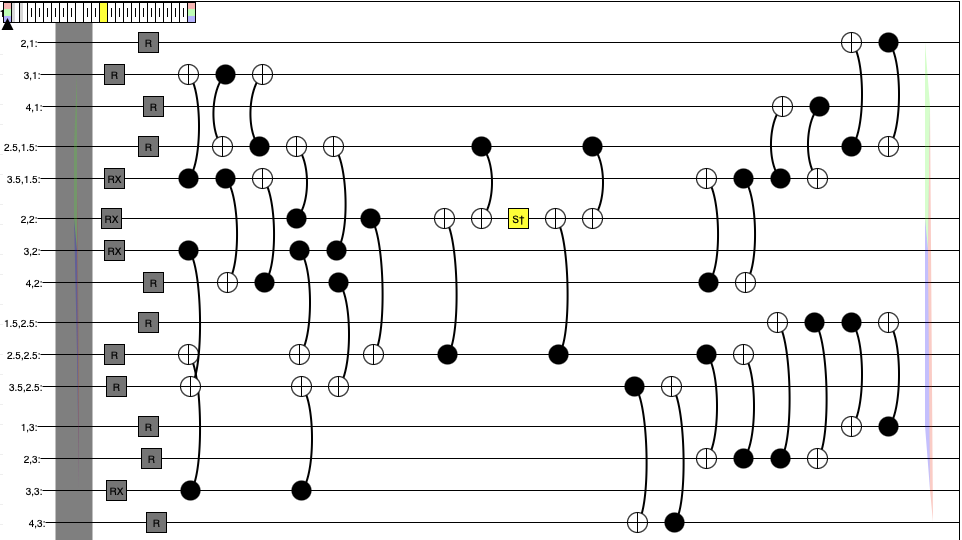
\includegraphics[scale=0.325]{stage1-injection-part1-modified-steane-code.png}
%		\begin{tikzpicture}[remember picture, overlay]
%			\node[anchor=south west, xshift=8pt, yshift=10pt, font=\tiny] at (current page.south west) {
%				\href{https://algassert.com/crumble#circuit=Q(1,3)0;Q(1.5,2.5)1;Q(2,1)2;Q(2,2)3;Q(2,3)4;Q(2.5,1.5)5;Q(2.5,2.5)6;Q(3,1)7;Q(3,2)8;Q(3,3)9;Q(3.5,1.5)10;Q(3.5,2.5)11;Q(4,1)12;Q(4,2)13;Q(4,3)14;TICK;R_7_6_11;RX_3_8_9_10;TICK;R_2_5_12_13_14_0_1_4;TICK;CX_9_6_8_11_10_7;TICK;CX_7_5_10_13;TICK;CX_5_7_13_10;TICK;CX_8_6_9_11_3_5;TICK;CX_8_5_13_11;TICK;CX_3_6;TICK;TICK;CX_6_3;TICK;CX_5_3;TICK;S_DAG_3;TICK;CX_6_3;TICK;CX_5_3;TICK;CX_11_14;TICK;CX_14_11;TICK;CX_13_10_6_4;TICK;CX_10_13_4_6;TICK;CX_10_12_4_1;TICK;CX_12_10_1_4;TICK;CX_5_2_1_0;TICK;CX_2_5_0_1;TICK}
%				{\underline{Click here to open this circuit in Crumble}}
%				};
%			\node[anchor=south west, xshift=8pt, yshift=2pt, font=\tiny] at (current page.south west) {
%				\href{https://algassert.com/crumble#circuit=Q(1,3)0;Q(1.5,2.5)1;Q(2,1)2;Q(2,2)3;Q(2,3)4;Q(2.5,1.5)5;Q(2.5,2.5)6;Q(3,1)7;Q(3,2)8;Q(3,3)9;Q(3.5,1.5)10;Q(3.5,2.5)11;Q(4,1)12;Q(4,2)13;Q(4,3)14;TICK;R_7_6_11_2_5_0_1_4_12_13_14;RX_3_8_9_10;TICK;CX_9_6_8_11_10_7;TICK;CX_8_6_9_11_7_5_10_13;TICK;CX_3_6_5_7_13_10;TICK;CX_3_5_6_4;TICK;CX_8_5_13_11_4_1_6_3;TICK;CX_13_10_5_3_1_0_4_6_11_14;TICK;CX_14_11_10_13_5_2_1_4;S_DAG_3;TICK;CX_10_12_1_3;TICK;CX_12_10_0_1_5_3;TICK;CX_2_5;TICK}
%				{\underline{Click here to open the compacted circuit in Crumble}}
%				};
%			\node[anchor=north west, xshift=4.5cm, yshift=-20pt] at (current page.north west) {
%				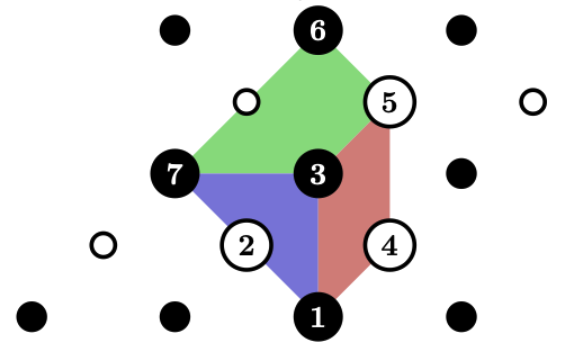
\includegraphics[scale=0.125]{t-state-injection-initial-layout1.png}
%			};
%			\node[anchor=north west, xshift=7.5cm, yshift=-20pt] at (current page.north west) {
%				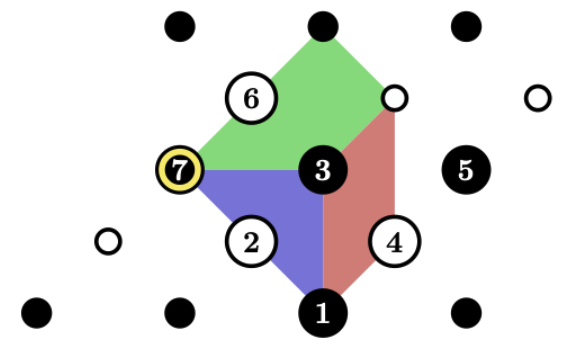
\includegraphics[scale=0.125]{t-state-injection-intermediate-layout1.png}
%			};
%			\node[anchor=south west, xshift=9cm, yshift=0.4cm] at (current page.south west) {
%				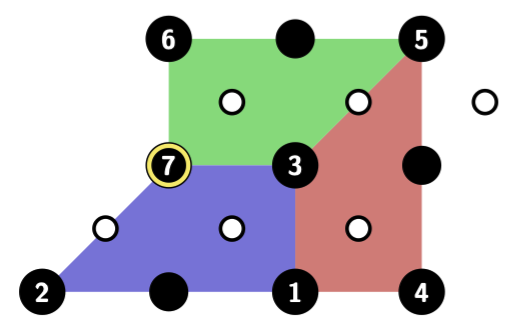
\includegraphics[scale=0.15]{t-state-injection-final-layout1.png}
%			};
%		\end{tikzpicture}
%	\end{frame}

%	\begin{frame}
%		\frametitle{Extra configurations for teleportation}
%		\vspace{0.4cm}
%		\begin{figure}
%			\centering
%			\scalebox{0.85}{
%				\begin{tikzpicture}
%					% Data qubits of the Steane Code
%					\coordinate (q1) at ( 2,-4);
%					\coordinate (q2) at ( 0,-4);
%					\coordinate (q3) at ( 2,-2);
%					\coordinate (q4) at ( 4,-4);
%					\coordinate (q5) at ( 2, 0);
%					\coordinate (q6) at (-2, 0);
%					\coordinate (q7) at (-2,-2);
%	
%					% Extra data qubits for forming GHZ states
%					\coordinate (dR) at ( 4,-2);
%					\coordinate (dG) at ( 0, 0);
%					\coordinate (dB) at ( 0,-2);
%					\coordinate (a0) at (-1,-1);
%					\coordinate (a1) at ( 1,-1);
%					\coordinate (a2) at (-1,-3);
%					\coordinate (a3) at ( 1,-3);
%					\coordinate (a4) at ( 3,-1);
%					\coordinate (a5) at ( 3,-3);
%	
%					% Plaquettes of the Steane Code
%					\fill[quantumR] (q5) -- (q3) -- (q1) -- (q4) -- (dR) -- cycle;
%					\fill[quantumG] (q6) -- (dG) -- (q5) -- (q3) -- (q7) -- cycle;
%					\fill[quantumB] (q2) -- (q7) -- (dB) -- (q3) -- (q1) -- cycle;
%		
%					% Plaquettes of the Surface Code
%					\fill[quantumR] (2,-6) -- (4, -6) -- (4, -7) -- (2, -7);
%					\fill[quantumR] (6,-6) -- (8, -6) -- (8, -7) -- (6, -7);
%					\fill[quantumB] (0,-6) -- (2, -6) -- (2, -7) -- (0, -7);
%					\fill[quantumB] (4,-6) -- (6, -6) -- (6, -7) -- (4, -7);
%					\fill[quantumB] (6,-6) arc[start angle=180, end angle=0, radius=1.0] -- (8, -6) -- cycle;
%					\fill[quantumB] (8,-6) arc[start angle= 90, end angle=0, radius=1.0] -- (8, -7) -- cycle;
%
%					\fill[quantumB, opacity=0.25] (2,-4) -- (4, -4) -- (4, -6) -- (2, -6);
%					\filldraw[quantumB, opacity=0.25] (q2) to[bend left=30] (0,-6) to[bend left=30] (q2);
%	
%					\node[data] at (dG) {\phantom{o}};
%					\node[data] at (dR) {\phantom{o}};
%					\node[data] at (dB) {\phantom{o}};
%	
%					\node[data] at (q1) {\large $\mathbf{1}$};
%					\node[data] at (q2) {\large $\mathbf{2}$};
%					\node[data] at (q3) {\large $\mathbf{3}$};
%					\node[data] at (q4) {\large $\mathbf{4}$};
%					\node[data] at (q5) {\large $\mathbf{5}$};
%					\node[data] at (q6) {\large $\mathbf{6}$};
%					\node[data] at (q7) {\large $\mathbf{7}$};
%					\node[circle, draw=yellow!95!black!75, line width=2pt] at (q7) {\phantom{o}};
%
%					\foreach \x in {-1, 1, 3}{
%						\foreach \y in {-1, -3}{
%							\node[meas] at (\x,\y) {};
%						}
%					}
%					\foreach \x in {-1, 3}{ \node[meas, opacity=0.35] at (\x,-5) {}; }
%					\foreach \x in {0, 2, 4, 6, 8}{ \node[data] at (\x, -6) {\phantom{o}}; }
%				\end{tikzpicture}
%			}
%		\end{figure}
%	\end{frame}

\end{document}